\PID \label{z:lpq_q_ampl} \mnImportant
За систем $H(s)$ дефиисан у задатку \ref{z:lpf_q}, за избор параметара 
$Q = 5$ и $\upomega_{\rm N} = 1\unit{\dfrac{krad}{s}}$,
\begin{enumerate}[label=(\alph*)]
    \item одредити граничне учестаности филтра $\upomega_{\rm g}$ такве да је
    $|H(\jj\upomega_{\rm g})| = \dfrac{\max|H(\jj\upomega)|}{\sqrt 2}$.
    \item Скицирати амплититудску фреквенцијску карактеристику датог филтра за параметре из претходне тачке. 
    \item Скицирати фазну фреквенцијску карактеристику. 
\end{enumerate}

\RESENJE 
(а) Амплитудска фреквенцијска карактеристика одређује се израчунавањем модула Лапласове трансформације 
на имагинарној оси, чиме се има 
\begin{equation}
    |H(\jj\upomega)| =
    \left|
    \dfrac{\upomega_{\rm N}^2 }{(\upomega_{\rm N}^2 - \upomega^2) + \jj\upomega\dfrac{\upomega_{\rm N}}{Q}} 
    \right| 
    =
    \dfrac{\upomega_{\rm N}^2}{\sqrt{  
        \left(\upomega_{\rm N}^2 - \upomega^2\right)^2 
        +
        \left(
            \dfrac{\upomega_{\rm N}}{Q} \upomega
        \right)^2
    }}
    \label{eq:\ID.freq}
\end{equation}
За скицирање графика испитаћемо асимптотско понашање дате фреквенцијске карактериситке. 
У случају када је $Q$-фактор довољно велики, тада је 
$\upomega\dfrac{\upomega_{\rm N}}{Q} \ll \upomega_{\rm N}^2 - \upomega^2$, изузев у непосредној околини 
$\upomega_{\rm N} \approx \upomega$, па је у том случају
\begin{equation}
    | H \bigl( \jj(\upomega \not \approx \upomega_{\rm N}) \bigr) |\approx
    \left|
    \dfrac{\upomega_{\rm N}^2}{\upomega_{\rm N}^2 - \upomega^2}
    \right|
    \approx \begin{cases}
        1 & \upomega \ll \upomega_{\rm N} \\[2mm]
        \dfrac{\upomega_{\rm N}^2}{\upomega_0} & \upomega \gg \upomega_{\rm N}.
    \end{cases}
    \label{fig:\ID.outband}
\end{equation} 
У случају непосредне околине $\upomega_{\rm N}\approx \upomega_{0}$, онда је доминантни члан у изразу
\ref{eq:\ID.freq} имагинарни део, па је онда 
\begin{equation}
    H \bigl( \jj(\upomega \approx \upomega_{\rm N}) \bigr) \approx 
    \dfrac{\upomega_{\rm N}^2}{\underbrace{\upomega}_{\mathclap{\approx \upomega_{\rm N}}}\dfrac{\upomega_{\rm N}}{Q} }
    \approx Q. \label{fig:\ID.maxval}
\end{equation}
Дефинисана граничну учестаност филтра одређује се на основу израза \ref{eq:\ID.freq}, нормирањем учестаности 
по $\upomega_{\rm N}$ увођењем нормиране граничне учестаности $w_{\rm g} = \upomega_{\rm g}/\upomega_{\rm N}$ добија се 
\begin{equation}
    \dfrac{\upomega_{\rm N}^2}{\sqrt{  
        \left(\upomega_{\rm N}^2 - \upomega_{\rm g}^2\right)^2 
        +
        \left(
            \dfrac{\upomega_{\rm N}}{Q} \upomega_{\rm g}
        \right)^2
    }} = \dfrac{Q}{\sqrt2} 
    \Rightarrow
    (1 - w_{\rm g}^2)^2 + \left( \dfrac{w_{\rm g}}{Q} \right)^2 = \dfrac{2}{Q^2}
\end{equation}
Добијена биквадратна једначина се решава чиме се добија нормирана гранична учесатност
$
    w_{\rm g} = \pm \sqrt{ \dfrac{2Q^2 - 1 \pm \sqrt{1 + 4Q^2}}{2Q^2}  }
$. 
У случају када је $Q$-фактор довољно велики, одбацивањем негативних решења, добијени израз
 се асимптотски може изразити као\footnote{У последњем корако примењује се апроксимација линеарним чланом Тејлоровог реда
 $(1 + x)^\upalpha \approx 1 + \upalpha x$, $x \ll 1$. }
\begin{equation}
    w_{\rm g} = \sqrt{ \dfrac{2Q^2 - \underbrace{\cancel{1}}_{\ll 2Q^2} \pm \sqrt{\underbrace{\cancel{1}}_{\mathclap{\ll 4Q^2}} + 4Q^2}}{2Q^2}  }
    \approx 
    \sqrt{
        \dfrac{Q^2 \pm Q}{Q^2}
    }
    \approx
    \sqrt{1 \pm \dfrac{1}{Q}} \approx 1 \pm \dfrac{1}{2Q}
\end{equation}
Граничне учестаности филтра су онда $\upomega_{\rm g} \approx \dfrac{\upomega_{\rm N}}{2Q}$, а ширина пропусног опсега је онда 
$\Delta \upomega = \dfrac{\upomega_{\rm N}}{Q}$. Из добијеног резултата може се приметити да са повећањем 
$Q$-фактора фреквенцијска селективност филтра расте, и у погледу резонантног појачања, и у погледу сужавања пропусног 
опсега.

(б) За потребе скицирања графика за задате параметре, можемо употребити одређене параметре асимптотског понашња. 
Пропусни опсег је $\Delta \upomega = \dfrac{\upomega_{\rm N}}{Q} \approx 0,2 \upomega_{\rm N}$.
На основу \eqref{fig:\ID.outband} за фреквенције испод доње граничне, карактеристика ће тежити јединици, док изнад 
горње граничне учестаности ће карактеристика тежити $\dfrac{\upomega_{\rm N}^2}{\upomega} 
= \dfrac{1}{\upomega_{\unit{krad/s}}}$. У пропусном опсегу, максимална вредност коју карактеристика достиже је 
према \eqref{fig:\ID.maxval} $Q = 5$. Границе пропусног опсега филтар пролази кроз тачке где је вредност 
$Q/\sqrt 2 \approx 3,5$.
График тражене карактеристике је нацртан на слици \ref{fig:\ID.crtez},
заједно са испрекиданом апроксимацијом моја може бити основа за ручно цртање. 


Ради потпуности, на слици \ref{fig:\ID.freq_resp} је приказан скуп различитих нормираних фреквенцијских карактеристика
за различите $Q$-факторе

\begin{figure}
    \centering
    %
    \begin{subfigure}[t]{0.45\textwidth}
        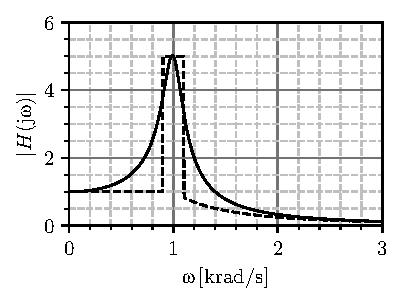
\includegraphics{fig/Q_ampl_approx.pdf}    
        \caption{Асимптотско понашање и скица амплитудске карактеристике филтра.}
        \label{fig:\ID.crtez}
    \end{subfigure}
    %
    \begin{subfigure}[t]{0.45\textwidth}
        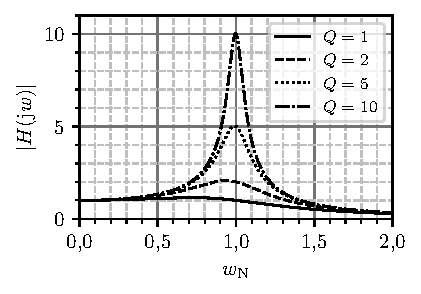
\includegraphics{fig/Q_razlicite_ampl_resp.pdf}    
        \caption{Нормирана амплитудска карактерситика филтра за различите $Q$-факторе}
        \label{fig:\ID.freq_resp}
    \end{subfigure}
    \caption{Уз решење задатка.}
\end{figure}